% DO NOT COMPILE THIS FILE DIRECTLY!
% This is included by the other .tex files.

\begin{frame}[t,plain]
\titlepage
\end{frame}

\begin{frame}
    \frametitle{\texttt{\$whoarewe} - MISP and CIRCL}
    \begin{center}
        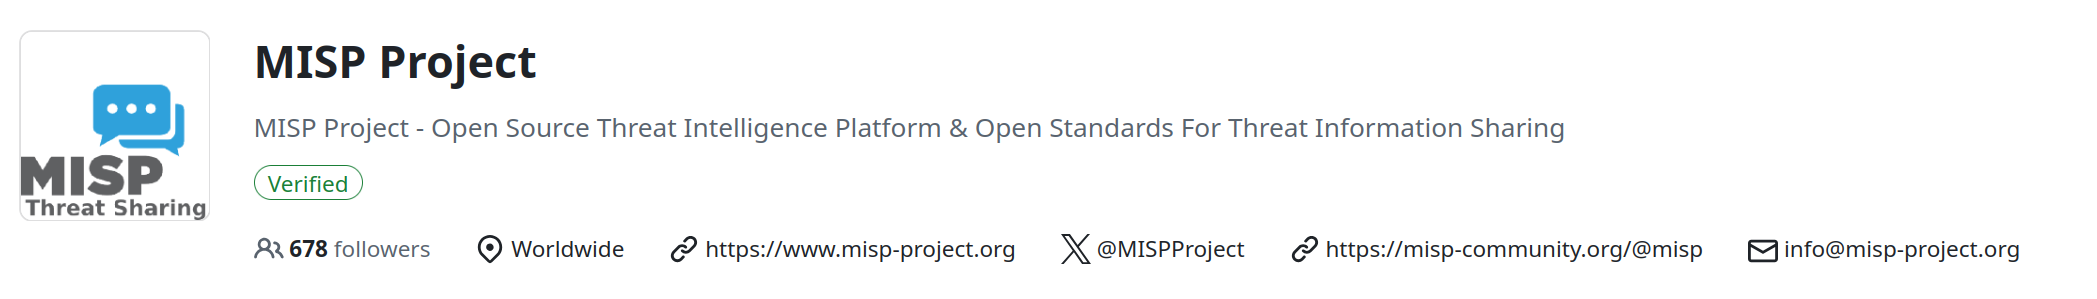
\includegraphics[width=1.0\textwidth]{misp-banner.png}
    \end{center}
    \begin{center}
        
\includegraphics[width=0.35\textwidth]{circl.png}
    \end{center}
    \begin{itemize}
        \item CIRCL is mandated by the Ministry of the Economy (under NIS 2).
        \item CIRCL leads the development of MISP.
        \item {\bf CIRCL manages multiple large MISP communities, enabling active daily threat intelligence sharing.}
        \item Funding comes from Luxembourg, various EU programs, and partnerships under EU/US agreements.
    \end{itemize}
\end{frame}

\begin{frame}
    \frametitle{Plan of this Session}
    \begin{itemize}
        \item MISP Intro: What it is, and what it can do
        \item Current state and Future of MISP
        \item How can MISP supports ISACs and its members
    \end{itemize}
    \vspace{1em}
    \begin{itemize}
        \item Building an information sharing community, lessons learnt and best practices\footnote{We published the complete guidelines in \url{https://www.x-isac.org/assets/images/guidelines_to_set-up_an_ISAC.pdf}}.
    \end{itemize}
\end{frame}

\begin{frame}
    \frametitle{What is MISP?}
    \begin{itemize}
        \item MISP\footnote{\url{https://www.misp-project.org/}} is a {\bf threat information sharing platform} ({\bf TISP}) that is free \& open source software
        \item Mature project that was started in 2012, and since then, has been following a community-driven development
    \end{itemize}

    \begin{center}
        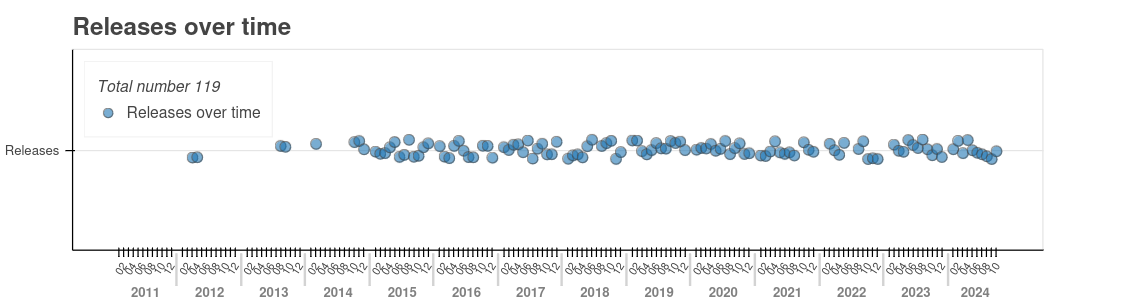
\includegraphics[width=0.99\linewidth]{release_overtime.png}
    \end{center}
\end{frame}

\begin{frame}
    \frametitle{What is MISP?}
    \begin{itemize}
        \item Used worldwide to manage and share threat-related information and intelligence.
	\item \textbf{Open-Source Commitment}: Users of MISP can rely on the tool remaining open source and never becoming closed source (autonomy of the users).
    \end{itemize}

    \begin{center}
        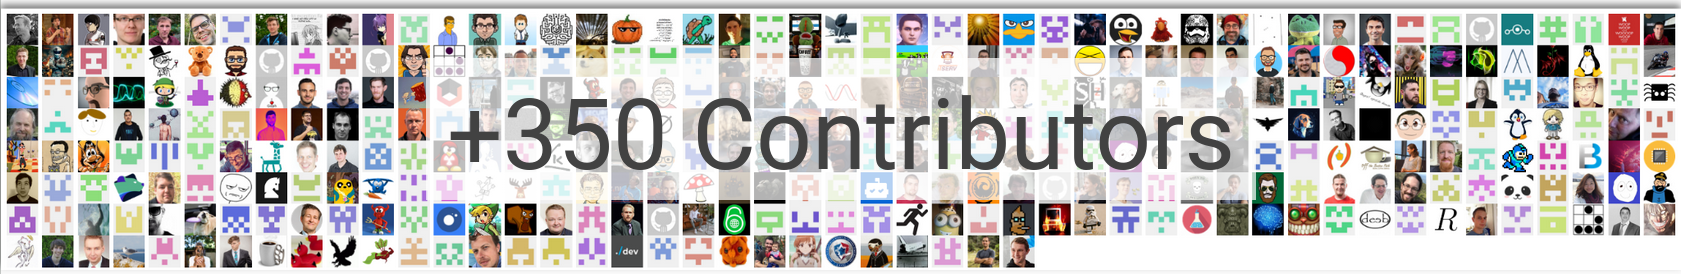
\includegraphics[width=0.99\linewidth]{contributors.png}
    \end{center}
\end{frame}


\begin{frame}
    \frametitle{What is MISP? (1)}
    \begin{itemize}
        \item MISP is a {\bf threat information sharing platform} ({\bf TISP}) that is free \& open source software
        \item A tool that {\bf collects} information from partners, your analysts, your tools, feeds
        \item Normalises, {\bf correlates}, {\bf enriches} the data
        \item Allows teams and communities to {\bf collaborate}
        \item {\bf Feeds} automated protective tools and analyst tools with the output
    \end{itemize}
\end{frame}

\begin{frame}
    \frametitle{Who is using MISP? (1)}
    \begin{center}
        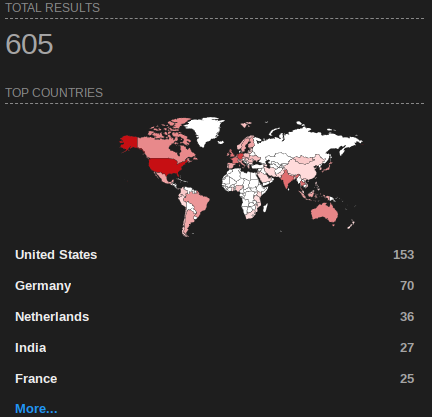
\includegraphics[scale=0.45]{misp-shodan.png}
        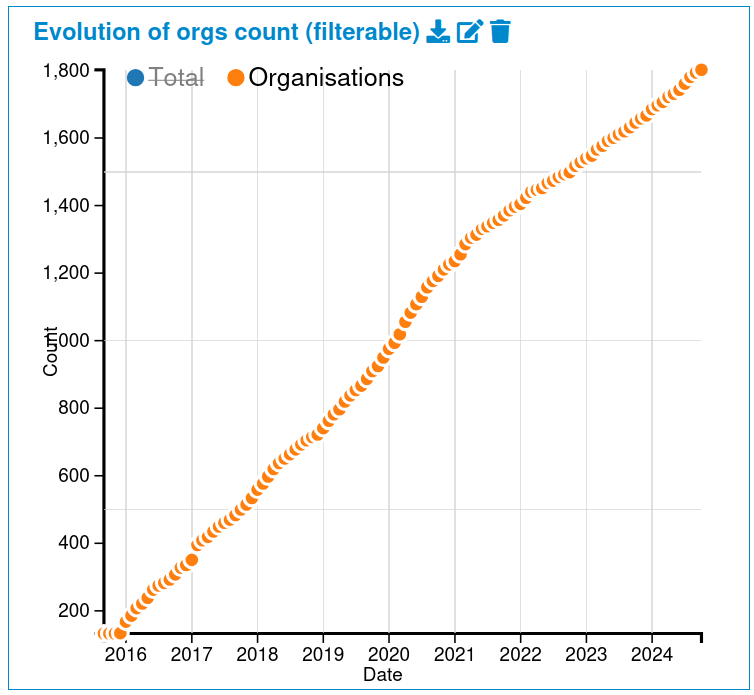
\includegraphics[scale=0.27]{org-count-misppriv.png}
    \end{center}
\end{frame}

\begin{frame}
    \frametitle{Who is Using MISP? (2)}
    \textbf{Communities:} Groups of users sharing within a set of common objectives and values.
    \vspace{1em}
    \begin{itemize}
        \item \textbf{Private Sector:} Financial, Manufacturing, Telecommunications.
        \item \textbf{Military and International Organizations:} NATO, military CSIRTs, national and governmental CERTs, etc.
        \item \textbf{Security Vendors:} Running their own communities or interfacing with MISP communities
        \item \textbf{Topical Communities:} Set up to tackle specific issues (e.g., COVID-19 MISP).
        \item \textbf{ISACs:} Serving various sectors such as Telecom, Retail, Aviation Traffic Control, etc.
        \item \textbf{Trusted Groups:} Operating MISP communities in island mode (air-gapped systems) or partially connected modes.
        \item \textbf{Law Enforcement Agencies (LEAs):} EUROPOL, INTERPOL, MISP-LEA, and more.
        \item \textbf{International Groups:} FIRST.org, MISP-Priv, and others.
    \end{itemize}
\end{frame}

\begin{frame}
    \frametitle{What is MISP? (2)}
    \begin{center}
        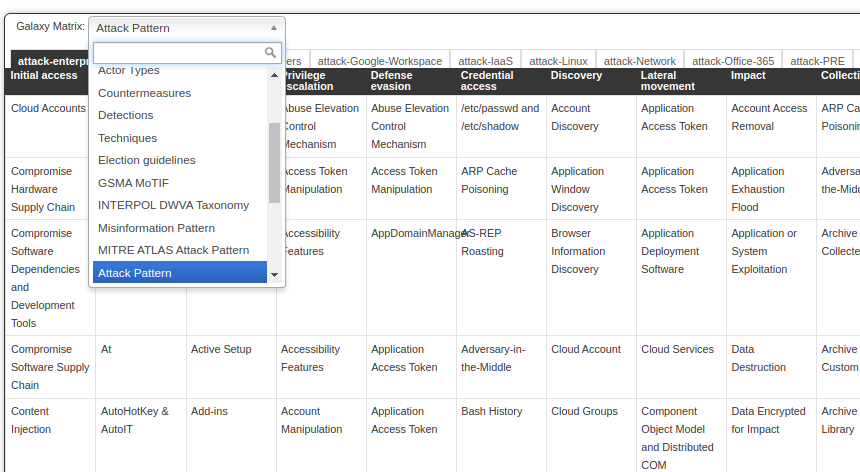
\includegraphics[width=1.0\linewidth]{galaxy-matrix.png}
    \end{center}
\end{frame}

\begin{frame}
    \frametitle{What is MISP? (2)}
    MISP is designed from the ground up to perform context-rich \textbf{threat intelligence}:
    \vspace{0.5em}
    \begin{itemize}
           \item {\bf Enrich} information with context and metadata
           \item Maps {\bf Threats and TTPs} (e.g MITRE ATT\&CK)
           \item Supports many {\bf standardized classification} marking
           \item Enables information {\bf curation} through automated quality checks
           \item Offers visualisation of threat {\bf relationships} and \textbf{technique} used
           \item Generates customizable {\bf threat reports}
           \item Allows creation of {\bf Dashboard} for trend analysis
    \end{itemize}
\end{frame}

\begin{frame}
    \frametitle{MISP Project Overview}
    \begin{center}
        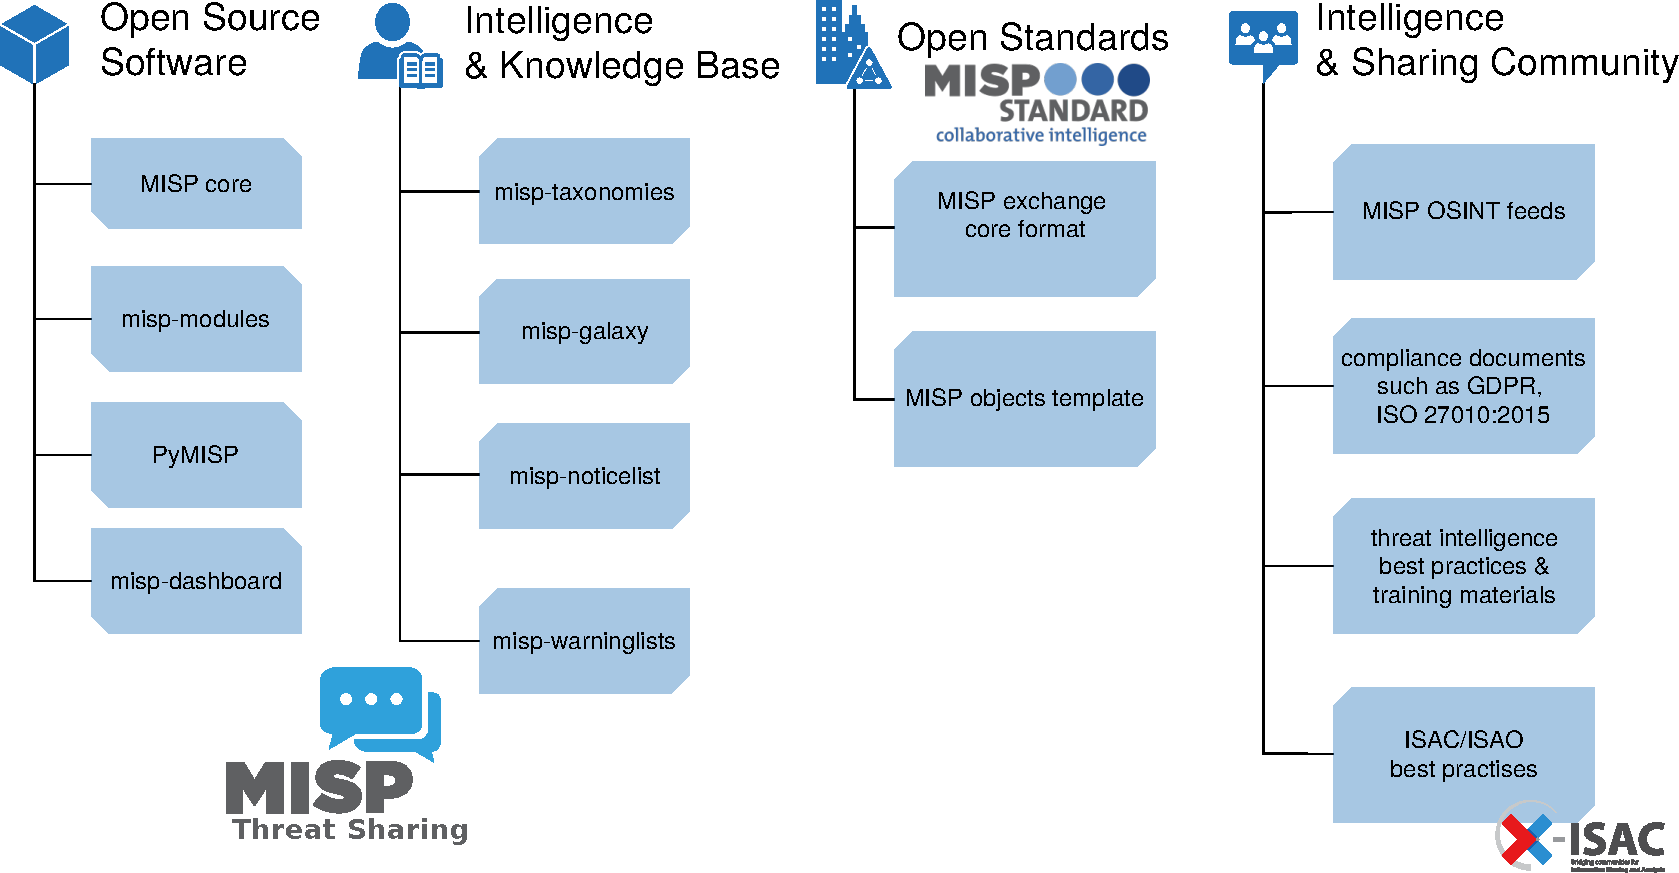
\includegraphics[width=0.85\linewidth]{misp-overview-simplified.pdf}
    \end{center}
\end{frame}


\begin{frame}
    \frametitle{Sharing in MISP (1)}
    \begin{center}
        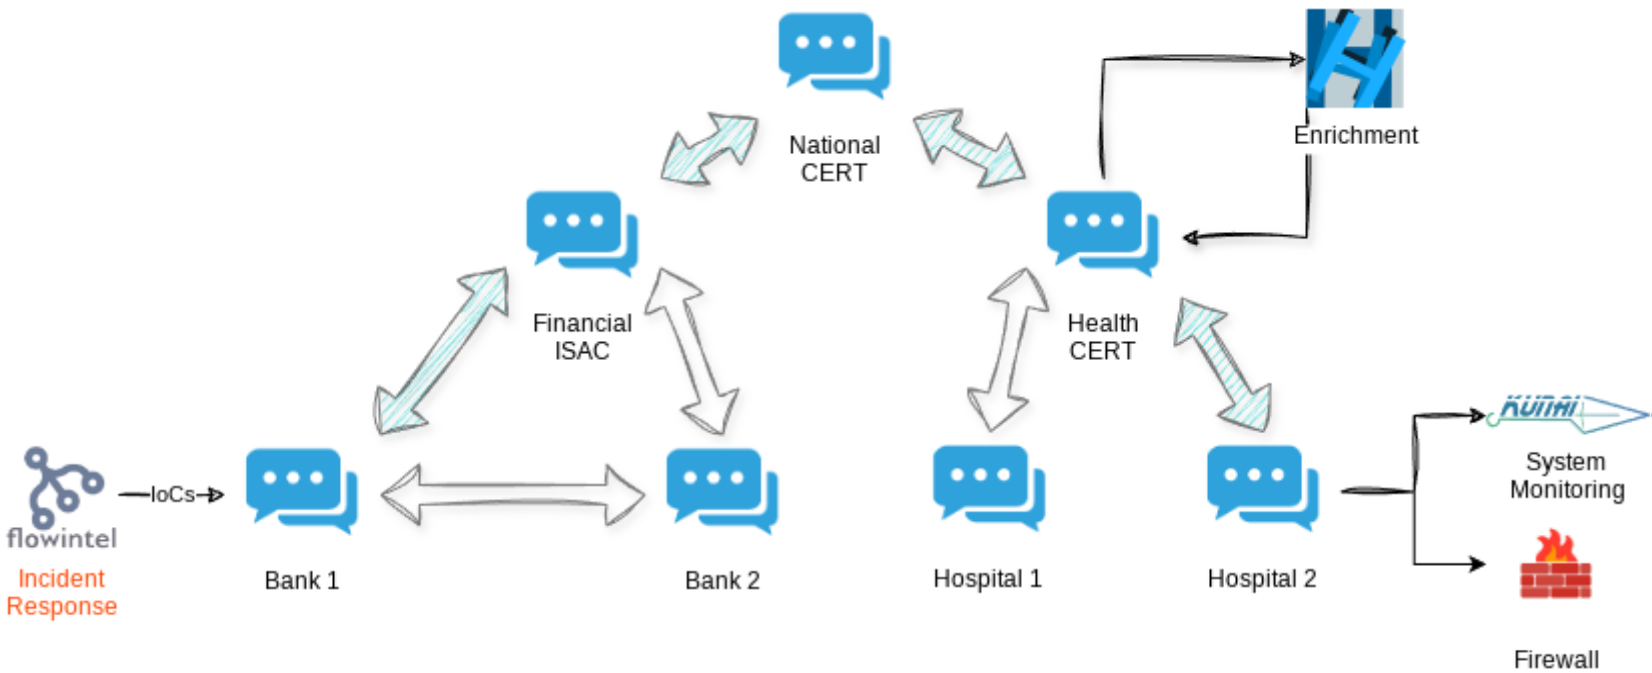
\includegraphics[width=0.99\linewidth]{misp-infosharing.png}
    \end{center}
\end{frame}

\begin{frame}
    \frametitle{Sharing in MISP (2)}
    MISP offers a wide range of \textbf{strategy to share information}:
    \begin{itemize}
        \item Many {\bf distribution level} offering granularity
        \item Sharing via distribution lists - {\bf Sharing groups}
        \item Incremental Synchronisation \& air-gapped sharing
        \item Feed system for ingestion \& generation
        \item User defined {\bf filtered sharing} for all the above mentioned methods
        \item Cross-instance information {\bf caching} for quick lookups of large data-sets
        \item Support for multi-MISP \textbf{internal enclaves}
    \end{itemize}
\end{frame}

\begin{frame}
    \frametitle{Information Quality Management}
    MISP has many features to help you manage and curate the data:
    \begin{itemize}
        \item \textbf{Correlating} data
        \item Feedback loop from detections via {\bf Sightings}
        \item {\bf False positive management} via the warninglist system
        \item {\bf Enrichment system} via MISP-modules
        \item {\bf Workflow} system to review and control information publication
        \item {\bf Integrations} with a plethora of tools and formats
        \item Flexible {\bf API} and support {\bf libraries} such as PyMISP to ease integration
        \item {\bf Timelines} and giving information a temporal context
        \item Full chain for {\bf indicator life-cycle management}
        \item {\bf Jupyter Notebooks} supporting common use-cases
    \end{itemize}
\end{frame}

\begin{frame}
    \frametitle{A Sample Curation Process in MISP}
    \begin{center}
        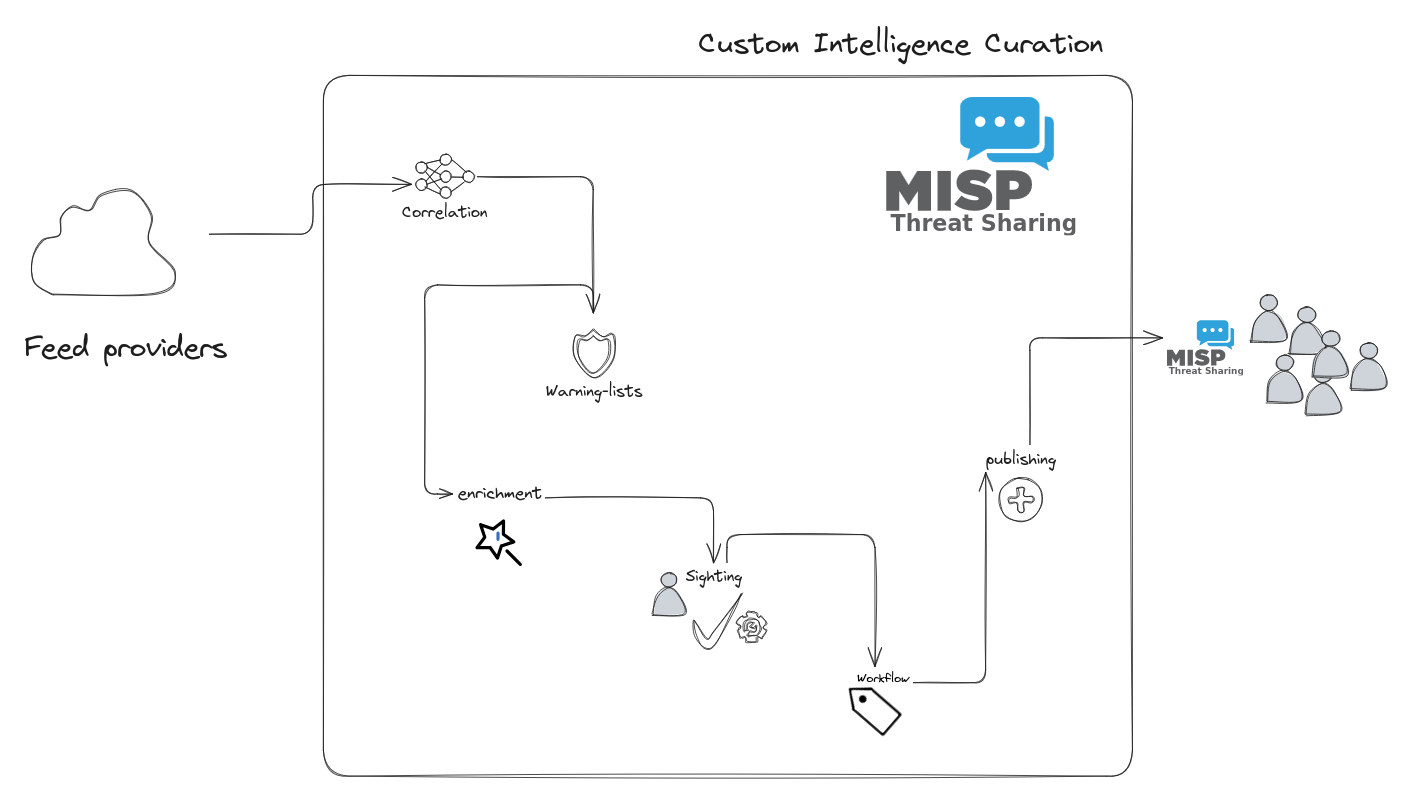
\includegraphics[width=0.84\linewidth]{curation.png}
    \end{center}
\end{frame}

\begin{frame}
    \frametitle{Flexible Data Format}
    \begin{center}
        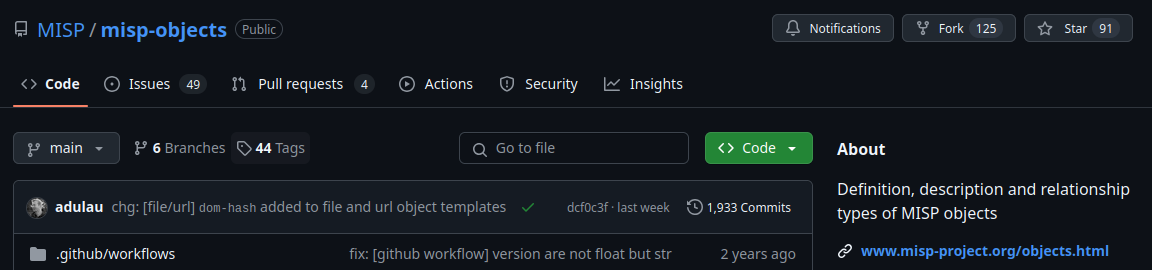
\includegraphics[width=0.99\linewidth]{misp-objects-repo.png}
    \end{center}
    \begin{itemize}
        \item Many Objects available to describe \textbf{any concepts}.
        \item Examples:
        \begin{itemize}
            \item IP address, URLs, file hashes, $\cdots$ 
            \item \textbf{Devices}: Mobile Phone, Sofwares, Devices
            \item \textbf{Payement}: Credit-cards, Transaction, Impacts
            \item \textbf{Vehicul}: Cars, Planes
            \item \textbf{Persona}: Passport, Person, Identity, PNR
            \item And \textbf{many more} $\cdots$
        \end{itemize}
    \end{itemize}
\end{frame}

\begin{frame}
    \frametitle{Integration and Automation ecosystem}
    MISP has many features to help you integrate various tools, processes and workflows:
    \begin{itemize}
        \item REST-full \textbf{API} \& \textbf{PyMISP}
        \item \textbf{PubSub channels} (ZeroMQ \& Kafka)
        \item \textbf{Enrichment} \& \textbf{Import/Export} service through MISP-modules
        \item \textbf{Workflow system}: Quick and easy automation based on trigger/conditions/actions blocks
    \end{itemize}
\end{frame}

\begin{frame}
    \frametitle{Information Quality Management}
    \begin{center}
        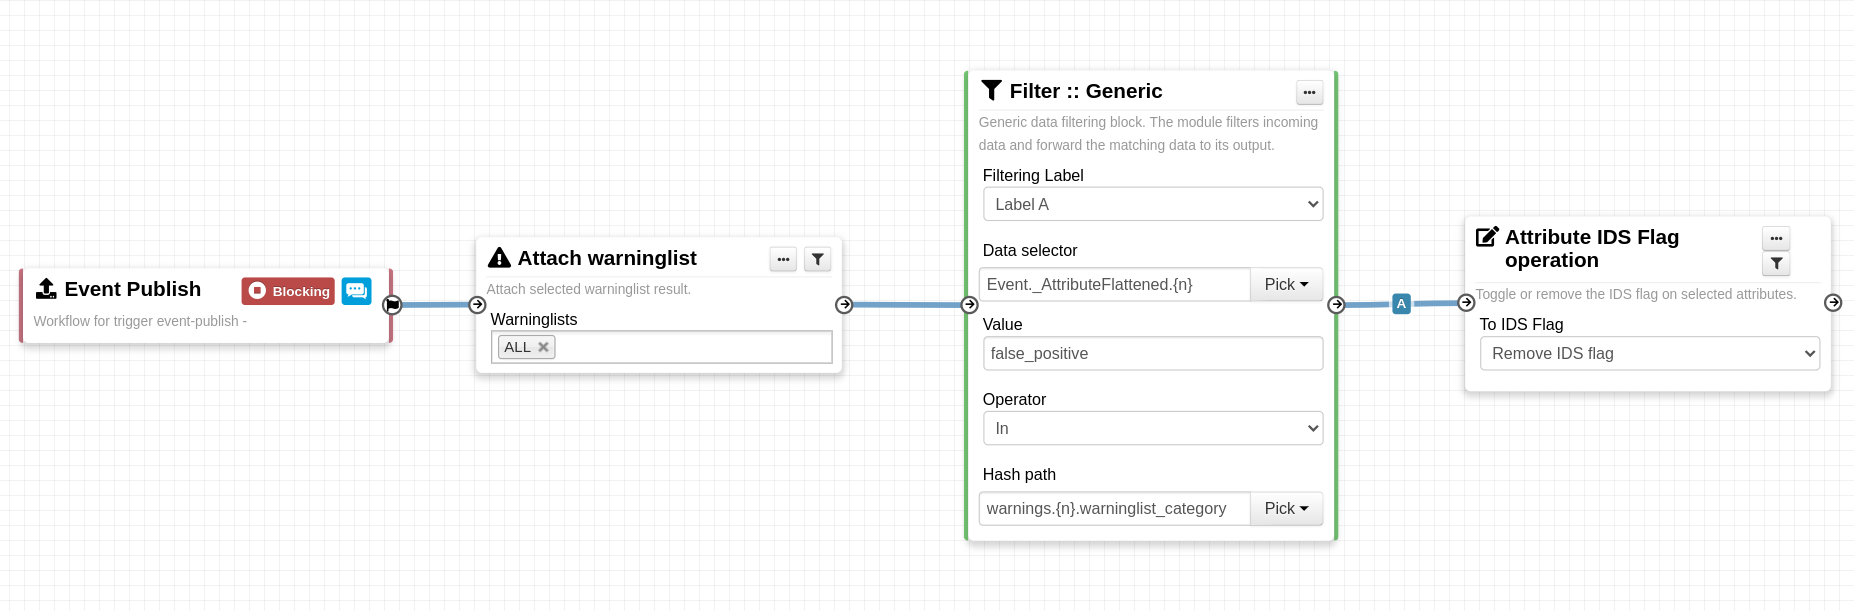
\includegraphics[width=0.99\linewidth]{wf-false-positive.png}
    \end{center}
    \begin{center}
        \textbf{Blueprint library} available on Github\footnote{\url{https://github.com/MISP/misp-workflow-blueprints}}
    \end{center}
\end{frame}

\begin{frame}
    \frametitle{Using the Power of the Community}
    MISP has many features to foster collaboration. To name a few:
    \begin{itemize}
        \item Proposals
        \item Analyst Data
        \item Delegation
        \item Sightings
        \item Extended Events
        \item Sharing-Groups
        \item $\cdots$
    \end{itemize}
\end{frame}

\begin{frame}
    \frametitle{Using the Power of the Community}
    \begin{center}
        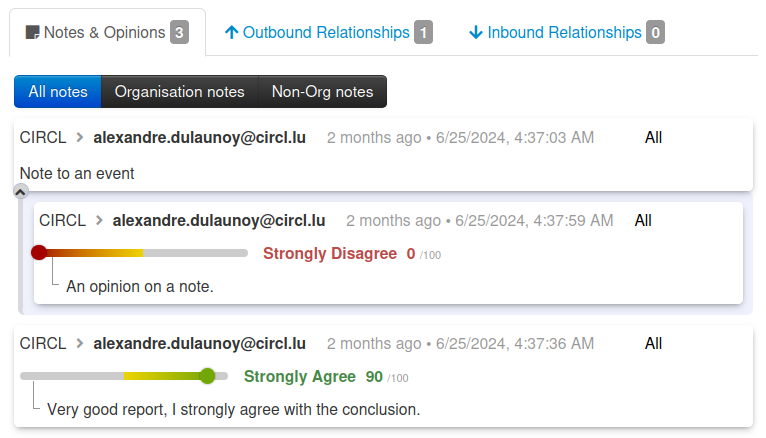
\includegraphics[width=0.85\linewidth]{analyst-data.png}
    \end{center}
\end{frame}

\begin{frame}
    \frametitle{Getting started: Joining/Running a sharing community using MISP}

    \begin{minipage}[t]{0.5\textwidth}
        \begin{center}
            \bf \Large As a Member
        \end{center}
        \begin{itemize}
            \item \textbf{Join} a "Hub" MISP instance
            \item \textbf{Host your own} MISP instance and connect to a "Hub"
        \end{itemize}
    \end{minipage}%
    \begin{minipage}[t]{0.5\textwidth}
        \begin{center}
            \bf \Large As a ISAC
        \end{center}
        Plan ahead:
        \begin{itemize}
            \item Estimate community \textbf{requirements and objectives}
            \item Decide on \textbf{common vocabularies}
            \item \textbf{Offer services} to your members
            \begin{itemize}
                \item Enrichment, Curation, $\cdots$
            \end{itemize}
        \end{itemize}
    \end{minipage}%
\end{frame}

\begin{frame}
    \frametitle{Success and Failure Stories in MISP Communities}
    \begin{itemize}
        \item We have supported various ISACs and sharing communities over the past years.
	\item Success largely depends on {\bf the dynamics} within the sharing community and how the rules are defined.
	\item Collaboration improves with {\bf contextualization practices} and {\bf well-established rules of operation}.
        \item Successful ISACs use MISP as a tool, customizing it to fit their specific needs.
    \end{itemize}
\end{frame}

\begin{frame}
    \frametitle{Incentives for Using Open Source}
    \begin{center}
        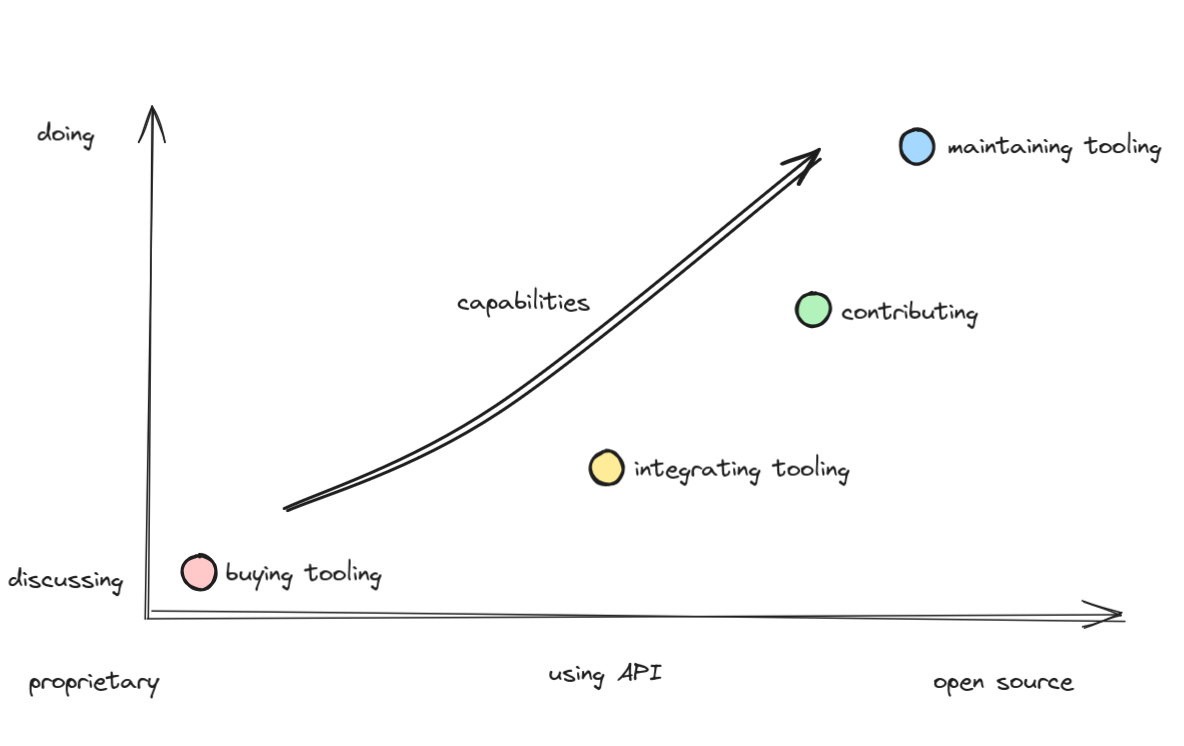
\includegraphics[width=0.8\linewidth]{opensource-csirt.png}
    \end{center}
\end{frame}

\begin{frame}
    \frametitle{Future of MISP: What's Ongoing}
    \begin{minipage}[t]{0.5\textwidth}
    \textbf{Medium Term:}
    \begin{itemize}
        \item We just released version \texttt{2.5}.
        \item Support for \texttt{2.4} will continue until 6 months after \texttt{2.5}'s release.
        \item Full feature parity and compatibility between \texttt{2.4} and \texttt{2.5}.
    \end{itemize}
    \end{minipage}%
    \begin{minipage}[t]{0.5\textwidth}
    \textbf{Long Term:} Major Version \texttt{3.0}
    \begin{itemize}
        \item Revamp front-end and aesthetics.
        \item Analyst-centric perspective.
        \item Improved search and analytics.
        \item Enhanced performance.
    \end{itemize}
    \end{minipage}%
\end{frame}

\begin{frame}
    \frametitle{CIRCL's MISP Professional Services (MPS)}
    \begin{itemize}
        \item We are comfortably funded to ensure the project's continued prosperity.
        \item MPS provides professional services and assists organizations seeking to secure support for MISP.
    \end{itemize}
    \vspace{1em}
    \textbf{CIRCL's Offering:}
    \begin{itemize}
        \item \textbf{Support Contract:} Prioritized issue resolution and expert guidance.
        \item \textbf{Training:} Tailored to the expertise level of participants.
            \begin{itemize}
                \item {\small Free onboarding MISP training for ISACs and their members.}
            \end{itemize}
        \item \textbf{Hosting:} Hosted on our infrastructure in Luxembourg (LU), available as virtual or dedicated instances.
            \begin{itemize}
                \item {\small OS and MISP maintenance, with early patching for security issues.}
            \end{itemize}
    \end{itemize}
\end{frame}

\begin{frame}
    \frametitle{Conclusion}
    \begin{itemize}
        \item MISP is just a tool—what truly matters are your \textbf{sharing and analysis practices}.
        \item MISP strives to meet the use cases of any community, from simple to complex ones.
        \item The MISP project combines \textbf{open-source software}, \textbf{open standards}, and \textbf{best practices} to make information sharing and analysis a reality.
    \end{itemize}
\end{frame}


\begin{frame}
     \frametitle{Contact}
     \begin{itemize}
	     \item \url{info@circl.lu} - \url{info@misp-project.org}
	     \item Open source software developed and used by CIRCL - \url{https://tinyurl.com/ISACTOOLING}
     \end{itemize}
\end{frame}


